\documentclass[IEEEtran,letterpaper,10pt,notitlepage,draftclsnofoot]{article}

\usepackage{nopageno}
\usepackage{alltt}
\usepackage{float}
\usepackage{color}
\usepackage{url}
\usepackage{balance}
\usepackage{enumitem}
\usepackage{pstricks, pst-node}
\usepackage{geometry}
\geometry{textheight=9.5in, textwidth=7in}
\newcommand{\cred}[1]{{\color{red}#1}}
\newcommand{\cblue}[1]{{\color{blue}#1}}
\usepackage{hyperref}
\usepackage{textcomp}
\usepackage{listings}
\usepackage{titling}
\usepackage{graphicx}
\usepackage{url}
\usepackage{setspace}

\graphicspath{ {images/} }

\definecolor{dkgreen}{rgb}{0,0.6,0}
\definecolor{gray}{rgb}{0.5,0.5,0.5}
\definecolor{mauve}{rgb}{0.58,0,0.82}
\lstset{frame=tb,
  language=c,
  aboveskip=3mm,
  belowskip=3mm,
  showstringspaces=false,
  columns=flexible,
  basicstyle={\small\ttfamily},
  numbers=none,
  numberstyle=\tiny\color{gray},
  keywordstyle=\color{blue},
  commentstyle=\color{dkgreen},
  stringstyle=\color{mauve},
  breaklines=true,
  breakatwhitespace=true,
  tabsize=3
}

% 1. Fill in these details
\def \CapstoneTeamName{   RoboSec}
\def \CapstoneTeamNumber{   50}
\def \GroupMemberOne{     Emily Longman}
\def \GroupMemberTwo{     Zach Rogers}
\def \GroupMemberThree{     Dominic Giacoppe}
\def \CapstoneProjectName{    Security for Robotics}
\def \CapstoneSponsorCompany{ Oregon State University}
\def \CapstoneSponsorPerson{    Vedanth Narayanan}

% 2. Uncomment the appropriate line below so that the document type works
\def \DocType{    %Problem Statement
        %Requirements Document
        %Technology Review
        %Design Document
        %Midterm Progress Report
        Research Paper
        }

\newcommand{\NameSigPair}[1]{\par
\makebox[2.75in][r]{#1} \hfil   \makebox[3.25in]{\makebox[2.25in]{\hrulefill} \hfill    \makebox[.75in]{\hrulefill}}
\par\vspace{-12pt} \textit{\tiny\noindent
\makebox[2.75in]{} \hfil    \makebox[3.25in]{\makebox[2.25in][r]{Signature} \hfill  \makebox[.75in][r]{Date}}}}
% 3. If the document is not to be signed, uncomment the RENEWcommand below
\renewcommand{\NameSigPair}[1]{#1}

%%%%%%%%%%%%%%%%%%%%%%%%%%%%%%%%%%%%%%%
\begin{document}
\begin{titlepage}
    \pagenumbering{gobble}
    \begin{singlespace}
      
\includegraphics[height=4cm]{coe_v_spot1}
        \hfill
        % 4. If you have a logo, use this includegraphics command to put it on the coversheet.
        %\includegraphics[height=4cm]{CompanyLogo}
        \par\vspace{.2in}
        \centering
        \scshape{
            \huge CS Capstone \DocType \par
            {\large\today}\par
            \vspace{.5in}
            \textbf{\Huge\CapstoneProjectName}\par
            \vfill
            {\large Prepared for}\par
            \Huge \CapstoneSponsorCompany\par
            \vspace{10pt}
            {\Large\NameSigPair{\CapstoneSponsorPerson}\par}
            {\large Prepared by }\par
            Group\CapstoneTeamNumber\par
            % 5. comment out the line below this one if you do not wish to name your team
            \CapstoneTeamName\par
            \vspace{10pt}
            {\Large
                \NameSigPair{\GroupMemberOne}\par
                \NameSigPair{\GroupMemberTwo}\par
                \NameSigPair{\GroupMemberThree}\par
            }
            \vspace{20pt}
        }
        \begin{abstract}
          In drones and other networked robotics there is a broad array of security vulnerabilities that can be leveraged in an attack.
          We will evaluate ROS to find as many of these security holes as we can and document them.
          The different vulnerabilities found will be categorized into malware, sensor hacks, network and control channel attacks, and physical breaches.
          For some of these exploits we may be able to implement solutions, which will also be documented.
          These findings and any solutions will be added to an ongoing academic effort to make robotics more secure.
        \end{abstract}
    \end{singlespace}
\end{titlepage}
\newpage
\pagenumbering{arabic}
\tableofcontents
% 7. uncomment this (if applicable). Consider adding a page break.
%\listoffigures
%\listoftables
\clearpage

\section{Introduction}
Robotics is still a relatively up and coming field and as most efforts in robotics are in pursuit of furthering capabilities, security has been left largely untouched.
Because of this many functioning, deployed robots have limited to no security in their internal systems, making them very vulnerable to attacks.
While the community developing robotics is still largely academic and there is little worry of being attacked, the security vulnerabilities still exist.
Soon robotics will become ubiquitous in society and hackers will exploit these vulnerabilities for personal gain.
There have already been reports of smart appliances being used for botnets, it's only a matter of time before drones and other robotics are similarly abused. \cite{ddos}
This project aims to eliminate some of this abuse before it begins.

\section{Problem Statement}
%ROS is known by many users to be insecure, but until now nobody had made any serious effort to document in which ways it is insecure.
%Our group undertook an exploratory effort to document ways we found it to be insecure as a starting point for what could be a more thorough documentation of the variety of ways it is insecure, for future research or development.
%This paper summarizes our findings.

Since robotics are continually in development and there is such a wide variety of devices, focus needed to be on a small subset of robotics to have any hope of making progress within a year. 
Because of this the Robotic Operating System (ROS) was chosen for this project.
These operating systems can be attacked at the driver level with malware, they can have the configuration files modified, and they can have data intercepted or spoofed in their internal communication subsystems.
We could also investigate the ability to spoof sensor data, such as the camera, IR guidance, accelerometer, or gyroscopic systems. 
Outside of the OS level there is a huge amount of room for exploitation in the communication and control channels used by networked devices. 
It's very important that we acknowledge all of these risks, since exploitation of them could be a big setback for global trust of robotics.

Essentially the problem is twofold; first a specific feature of a specific device needs to be isolated, and then that feature needs to be broken, and all work documented.
This could be a crucial improvement for the use of robotics running ROS in a wide variety of sectors.
The military uses and plans to use them widely, and for them more than anyone they need to be as secure as possible.
Amazon and other commercial shipping companies have a vast use of robotics, and we've all heard about their plans for delivery drones, which are a huge security risk.
If consumers think these will be abused they won't trust this upcoming technology and it will be slowly or never adopted, which will make companies hesitant to invest in their development.
Consequentially, the world as a whole will be slower to advance robotic technology.
Hopefully our work in securing robotics can help to better develop consumer trust in this emerging technology.

\section{Literature Review}
This project would have been much more difficult without a variety of documentation and previous research into the security of ROS and robotics in general.
One paper that was widely used in the creation of our project basis was "A Preliminary Cyber-Physical Security Assessment of the Robotic Operating System (ROS)". \cite{mainROS}
This article was written by a group of researchers who created a honeypot robotic system and brought it to DefCon 20 to let hackers there exploit it as they could.
This lead the researches to be able to recored a range of attack vectors from a wider variety of minds.
They also used a number of their own methods to study what was being done, such as examining the packets being sent and received through wireshark, visualizing the effects with hardware, and using Backtrack Linux.
Their work provided starting points for many different ways to attack the system, and for cataloging the effectiveness of each different type, relative to the others.
The inspiration from this paper laid a groundwork for the threat models that would be created here, and for the exploratory structure that was followed.

Another particularly useful paper was written by Bernhard Dieber et al, which discussed security on the application level of ROS.
It provides great insights for the problems with authentication and data integrity that are present in ROS. \cite{App}
This article helped to provide guidance for that portion of our model, and was foundational in the understanding of how the application level interacts with the rest of the system, from a security standpoint. 
A similar paper entitled "ROS: an open-source Robotic Operating System" was vastly useful in the planning of this project, as it gave a detailed overview of the system from a research standpoint.
While the official site and documentation of ROS was absolutely invaluable, this paper provided us with a third party assessment of the system and how all portions work together.
Without a thorough understanding of this research would be much more difficult. \cite{Open}
 
The last of the papers that were used extensively in the overall planning and implementation of this project was one discussing the SROS project.
This project is very closely aligned with ours in that they are working to bring better security to ROS in its most vulnerable sectors.
The areas in which this project most wanted to provide security were some of the first that our project investigated. 
Specifically it provided insight into the access control policies needed in ROS, the insecurity of the communication channels, and they way in which processes are handled. \cite{Sros}

When looking for background information for specific exploits that would be created, a lot of other research papers, journal articles, and security presentations were examined.
These are referenced and discussed within each of packages to which they contributed.

\section{Threat Model}
A key element to our project is being able to accurately find vulnerabilities or identify areas where they are likely to be.
One of the best ways to do this in an organized way that can be later referenced is with threat modeling.
Adam Shostack has a well defined method for doing this, which was followed to develop the model for this project. \cite{TMDS}

An important thing to note is that ROS is middleware, which means it sits between the base Linux OS, and the application level.Typically there is little focus on security because middleware like this needs to be lightweight. 
Without any specific security measures taken, there is room for all manner of attacks. To try to tackle them, the vulnerabilities were broken into the three categories of the CIA Triad \cite{CIA}:
\begin{itemize}
  \item Those affecting the confidentiality of data
  \item Those affecting the integrity of data
  \item Those affecting the availability of data
\end{itemize}

A threat model was created to visualize these three categories. It serves as a roadmap for the research and can be looked back on at any time.
The model below in Figure 1 is organized as a tree, with the three main branches being the three components of the CIA triad (Confidentiality, Integrity, and Availability).
This way one can look at our threat model, decide if their concern is one of confidentiality, integrity, or availability, then examine the vulnerabilities in that category.

\begin{figure}[H]
    \centering
    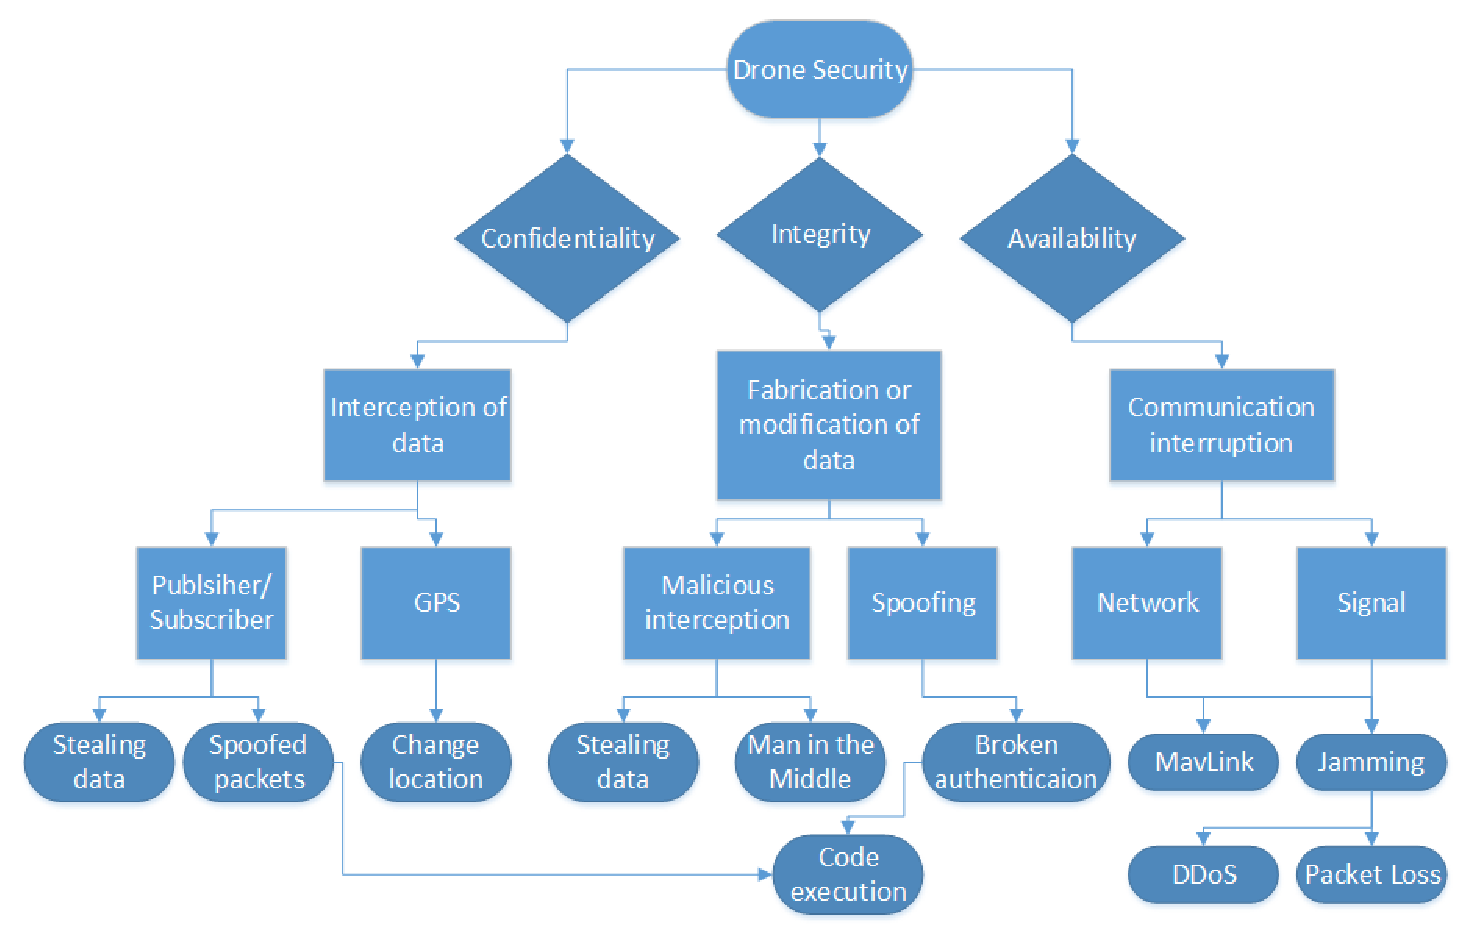
\includegraphics[width=\textwidth]{model.eps}
    \caption{A view of the attacks that are viable against the ROS system}
\end{figure}

In this figure the top levels are the three sectors of the CIA Triad, which branch into the attack types within each.
Below that level are the rectangular examples of vulnerabilities of that type.
Lastly the bottom tier nodes are attack type examples.

\section{Packages and Solutions}
As mentioned above, the exploits written were meant to cover a lot of ground topic wise.
Some are based on the same vulnerability, while others are more distinct.
Specific packages have been chosen below to represent each of the notable categories of attack.
These range from resource consumption, to network sniffing and spoofing, and to OS level exploitation.
In the Analysis section below there is a table showing where in the CIA triad each of the exploit packages falls.

\subsection{Eavesdropper}
Called Malpac in the repo, this is a very simple package. It has 2 nodes, one that publishes a string every couple seconds, and 
a subscriber that takes that message and prints it to stdout. There is also a third “malicious” node which also subscribes to 
the publisher and prints the same message with a slight modification to stdout as well. While not that malicious in this case, 
the general principle can be used to receive and change any published data, including sending said data to other computers 
using the ROS subscriber/publisher system and compromise the original data’s integrity.
For example, if you had a drone doing aerial reconnaissance of an area and transmitting the images back to a base, this kind of 
system would be able to intercept those images.

This package was one of the first ideas implemented so it started in one of the most obvious places within our model, the Publisher/Subscriber system.
It falls under the confidentiality section of the threat model because it steals data that would be best kept confidential. 
Although not particularly sophisticated, the unencrypted nature of this communication channels means it doesn't need to be. 
With little difficulty it demonstrates how trivial it is for a malicious actor to listen in on communications between nodes and steal useful information.
This is expanded upon in later packages which take this easily gained information and use it spoof the system.

\subsection{Forkbomb}
This package is a forkbomb.
As stated previously there is no process monitoring or control native to ROS, so this is a very simple forkbomb. All it does is 
do a little math to slow things down a bit, then call itself 8 times and exit.
Eventually there are enough processes to clog the CPU and cause a kernel panic, bringing down the robot.
In theory, as long as there is no existing form of process management, this would kill any robot with enough time, which has 
obvious use cases.

Forkbombs like this one work to fill up processing resources so that the system has a much harder time scheduling legitimate processes. 
This is essentially denial of service, which falls into the availability branch of attacks, since the system resources are rendered unavailable when done successfully.
Distributed denial of service (DDoS) attacks are becoming more and more common in Internet of Things devices, and this package shows how it easy is to do something similar within a ROS device.

\subsection{Network Bomb}
This exploit temporarily disables the operating system's wireless networking capabilities.
For a robot dependent on wireless communication for control or navigation, this has some rather obvious consequences.
Depending on how the robot handles the lack of networking it could do anything from fall out of the sky to automatically
returning home. It could also permanently disable the wireless networking with a small tweak, which would make the only 
fix to physically capture and wire back into the robot to fix the networking. 
Either way, if one's robot is dependent on wireless networking, it will be downed for a bit.

Much like the forkbomb, and similarly named, the network bomb is also an exploit that reduces the availability of the system resources.
Specifically this one uses up the communication resources, which cuts it off from the control center and potentially allows an attacker to take over.
This was developed to flesh out the DoS portion of the model, so that the forkbomb focuses on consuming internal resources, while this one consumes the network.

\subsection{Fibonacci}
This one is actually our Client, Vee's package. It does a naive recursive implementation of the calculation of Fibonacci
numbers, and tries to calculate the 100000th number. It either takes a long time, or stack overflows and crashes, neither 
of which being terribly great results and both using a fair amount of system resources. As such it has the potential to 
bring down the system, depending on how exactly python handles the recursion involved, or at least be a waste of resources 
for a bit.

This was one of the first packages in existence and served as somewhat of an example of what future packages might look like. 
It was also why a number of the earliest packages focused on resource consumption and computationally intensive work.
Even if this isn't the most creative or greedy way to reduce availability, it serves as an elegant and classic proof of concept for availability focused packages.

\subsection{Local Folder}
This package just creates and then deletes a local folder. In theory it can delete any user level folder, which may include
program files or ROS nodes or maybe just something important locally. If it has super user permissions then it could go so
far as delete system directories or the like, but that is not guaranteed. Either way it can probably delete something that
the user would rather it not.

This package is yet another one that compromises the availability of the system. 
While it could be used to remove mundane things, it also would be capable or deleting crucial folders, giving it the potential to be quite dangerous.
It is an interesting approach to the availability side of attacks, since they often use tactics that increase the load on the system, rather than removing critical portions.

\subsection{Node Replacement}
Consisting of 2 parts, this includes one package which launches a publisher that publishes a string every couple seconds and a 
subscriber that takes that string and prints it to stdout.
The other one runs a package that kills the subscriber from the 1st package, and replaces it with its own subscriber with the 
same name that prints a modified message to stdout.
At the time we thought the node would be indistinguishable from the previous node besides the different message, but it turns 
out that ROS silently assigns each publisher and subscriber its own unique ID and is in fact quite noticeable.
It might be hard to notice by an inattentive user, assuming they do not notice the slight hiccup where the old subscriber dies 
and is replaced, so it still has potential to be a threat or phone home.

This exploit works on the integrity portion of the tree, by doing a rudimentary form of a man in the middle attack.
The system is somewhat fooled into thinking that the new node was the original publisher and takes information from it.
While the unique ID makes this package not useful as is, it still provides a solid proof of concept for the idea. 
It was also used as a starting point for some later iterations of the same concept. 

\subsection{Costly Sorting}
This is a package that performs bogo-bogo sort. \cite{bogo}
Bogo-bogo sort is an extremely inefficient sorting algorithm that performs a random shuffle to sort a list, recursively.
While it is not particularly system intensive, the sort for a list with a mere 10 elements can take on the order of days.
The goal of this package was not to be directly malicious but more of a lurking threat; it shows that ROS also does not check 
for any particularly long running processes, which allows for a variety of actual threats. It also wastes some CPU time.
The best example is an attack that lies dormant until signaled to do maximum damage, or one that waits for a specific process 
to kill it.

This package falls into the availability spectrum, as it uses a processing intensive sorting algorithm to eat up computing resources.
As stated above it also serves as proof of concept for the fact that ROS doesn't cut processes off after any certain amount of time.
This same idea can be used in many different ways, with different types of resource consumption being called at specific times to deny service to legitimate actions.

\subsection{URI Change}
This is a package that changes the ROSMASTER URI to an arbitrary one, and starts a new ROS master to match.
The URI is basically where packages check for the ROS master node, which is the master in the ROS master/slave system.
ROS master manages nodes, and the publisher/subscriber system between nodes as its 2 main duties.
As such, changing the URI and starting a new ROS master node means that all new nodes will talk to the new ROS master as 
opposed to the old, which could allow for some interesting node management or fiddling with the publisher/subscriber system.
The ROSMASTER URI can also be set to a remote machine if it setup correctly as well, which means you could have a compromised 
robot respond to a remote ROS master node as well, allowing an attacker to control the robot remotely.

\subsection{Pkiller}
This simply pkills (process kill, for those unfamiliar) all processes with ROS in the name.
This will at least kill ROS master, and maybe some other related ROS processes, but killing ROS master also kills all the nodes currently being managed by ROS master, so it will also kill all ROS processes on the system.
This has the obvious effect of bringing the robot to a halt, and has the potential of doing major damage.
Just image if a drone carrying an explosive payload fell out of the sky because its control system suddenly stopped.

This attack removes availability by killing key processes, but can also be used to kill something legitimate and then replaces it with a malicious process, which would be an integrity attack.
Much like many of the previous packages, this one was created to further explore the ways in which system control and accessibility can be taken away, with something other than just resource consumption.

\subsection{Massive Download}
This package uses wget to attempt to download all of Wikipedia.
It probably will not succeed, unless the robot has enough disk space to hold all of Wikipedia, but it will fill the disk up to 
the limit. This can cause a number of issues depending on what else needs disk space, but it is sure to cause some sort of 
issue. If nothing else it will prevent any more ROS processes from being launched, as ROS master does some record keeping for 
each process and will need a little disk space for that purpose.

This package works to break down the availability of the system by filling up disk space, which mean it can stop legitimate data being stored.
This is an interesting approach to denial of service in that it doesn't have to be continuous but rather only needs to be run once.
After having done this there are a number of routes the attacker could follow, such as replacing this downloaded data with their own malicious files, or even making the initial massive download contain malware to serve whatever purpose they desire.

\subsection{Root Dump}
This package dumps your filesystem to a remote machine, currently a dummy address. If you had something confidential on the
robot, it is now in the hands of some other party, assuming your network connection did not die mid-transfer or something.
If your drone had those top secret recon images, or maybe the drone's code itself was supposed to be a secret, they could
potentially be in the hands of some unknown party.

This package is one of the first in the confidentiality portion of the tree.
It uses surprisingly simple tactics to give a malicious person access to a copy of the entire file system, leaving them free to peruse the contents and use them.
This goes to prove just how big even basic file encryption on ROS would be, since that would prevent this from being a viable attack.

\subsection{Uninstaller}
This one, assuming your ROSMASTER was run with root privileges and is on a Linux distribution that uses apt-get as its package
manager, uninstalls ROS from the robot. The robot's operations will be unaffected until next boot as the ROS binaries will be 
loaded into system memory, but on reboot or if ROS is killed and restarted in some other way, ROS will no longer be there.
Especially bad if the ROS install was customized, as one would have to redo all those configurations all over again...

This attack is almost the exact opposite of the previous one.
It uses system capabilities to remove ROS itself, which is essentially the ultimate shut down.
Although, as stated above, this wouldn't actually take effect until the next time the system was booted up, it still serves as a very effective way to deny someone access to their robotic control by rendering their system completely unavailable.

\subsection{Start WW3}
This pings (what the team knows to be, but can not directly confirm) a North Korean IP address. 
While it has no direct effect on the system, alerting North Korea to your presence is not exactly a great idea in the current political environment, and has a good chance of getting one on a watchlist. 

This package was written mostly for fun, since it doesn't do much from a research standpoint.
It's hard to even classify where it would fit into the CIA Triad.
It seems to hurt the person who owns the ROS device more than the device itself.
In that case it would be quite effective for targeting someone and getting them investigated or arrested or in some way causing them legal and diplomatic problems.

\subsection{Bitcoin Miner}
This package attempts to install a bitcoin mining service on the robot.
It does currently need superuser permissions for this, as it does need to use apt-get, which means that ROSCORE 
needed to be run as a superuser so that this child process would have those permissions as well.
If the install succeeds however, then you have a bitcoin miner using CPU time for someone else’s monetary gain, and with a 
little more work could be further configured to have the miner run at boot as a system process, but for the purposes of the 
package it was good enough as is.

Bitcoin mining is also a more fun type of package, but it does also serve to reduce the availability of the system resources since its mathematically intensive.
It also somewhat touches upon the other two portions of the triad in that it compromises the system's integrity, and reveals some potentially confidential system information.

\subsection{ROSless Listener}
Here was an attempt to abuse how ROS subscribers and publishers really worked outside of ROS.
All subscribers and publishers actually communicate through a shared TCP/UDP socket controlled by ROS master, and the general 
idea was to make a non-ROS socket to communicate with the ROS socket, subscribe to a known publisher on the ROS machine, and 
print whatever they published as plain text to stdout.
In short, something like the first malpac, but going around ROS to do so. Unfortunately ROS uses TCP/UDP with a special header encoding that makes this difficult, as to communicate any publisher or subscriber you need their unique ID, which is assigned to them by ROS master at their launch. And to get said ID, you need to do some handshaking with ROS master, which turned out to be a bit beyond our technological capacity and time constraints.
We believe it is still possible to achieve this, but to do so would require a better working knowledge of sockets and more 
investigation into the handshake protocol used by ROS master.
While the documentation is available online, specifically on the technical overview page of the official ROS site \cite{ROS}, it was just a little too much for the team with the time we had. Malpac ROS is similar to this, but differs in that Malpac ROS 
still uses ROS to achieve this goal, while this package aimed to bypass ROS entirely.

\subsection{Linux Kernel Exploitation}
This package contains two scripts, a memory hook and a stack smasher.
The first, the memory hook, is actually a Linux kernel exploit, and doesn't use ROS itself, but ROS commonly sits atop Ubuntu or Ubuntu-based linux systems. \cite{kern}
This package does a simple memory hook into the syscall table, which allows the script to make changes to whichever syscalls it wants once it finds the syscall table memory address. \cite{hook}
This is done by changing the pointer to the function of an existing syscall and replacing it with a pointer to a malicious function.
This is the kind of script that would likely be secondary to one of the network attacks. One of those might be used to get into the system, and could then install LKMs like this one. Since it operates at the kernel level in Linux, ROS would have no way of ever knowing something was amiss, which renders this a very insidious threat.

The second script, the stack smasher, provides a basic proof of concept (PoC) for stack smashing. \cite{SS}
This is a form of buffer overflow attack which has been used reliably for a very long time to gain unauthorized access to a system.
It works by leveraging the overflow to push its way into privileged space and then execute some form of malicious code once it has entered that area of the stack. \cite{SS2}
This specific script is a small scale buffer so better demonstrate the idea.
To use a simple approach like this, one needs access to the environment variables of the system so it's not perfect.

Both of these different OS exploits affect the availability and the integrity of the system.
They both remove the availability of their area's primary functionality on the way to modifying it and damaging the integrity.
Some confidentiality is also lost in the process, but it's a negligible effect.
The idea for both of these came primarily from subject matter covered in the Defense Against the Dark Arts class, and because the underlying kernel was an area of the system that had yet to be touched.

\subsection{GPS Exploitation}
The exploits in the category work with the GPS or Mavlink protocol.
Specifically the GPS package uses both spoofing and man in the middle to trick a drone into thinking it is the home base, and can misguide it.
This is done by sniffing for drone network information, and then leveraging that to send spoofed landing data via UDP.
The Mavlink script follows the same idea, but it was never able to reach a point of development beyond simply sniffing for the information and positioning itself as a node in the middle.
With better documentation and a system with which to reliably test it the Mavlink script could grow to the point of the GPS one.

\subsection{ROS Broken Authentication PoC}
\begin{figure}[H]
  \centering
    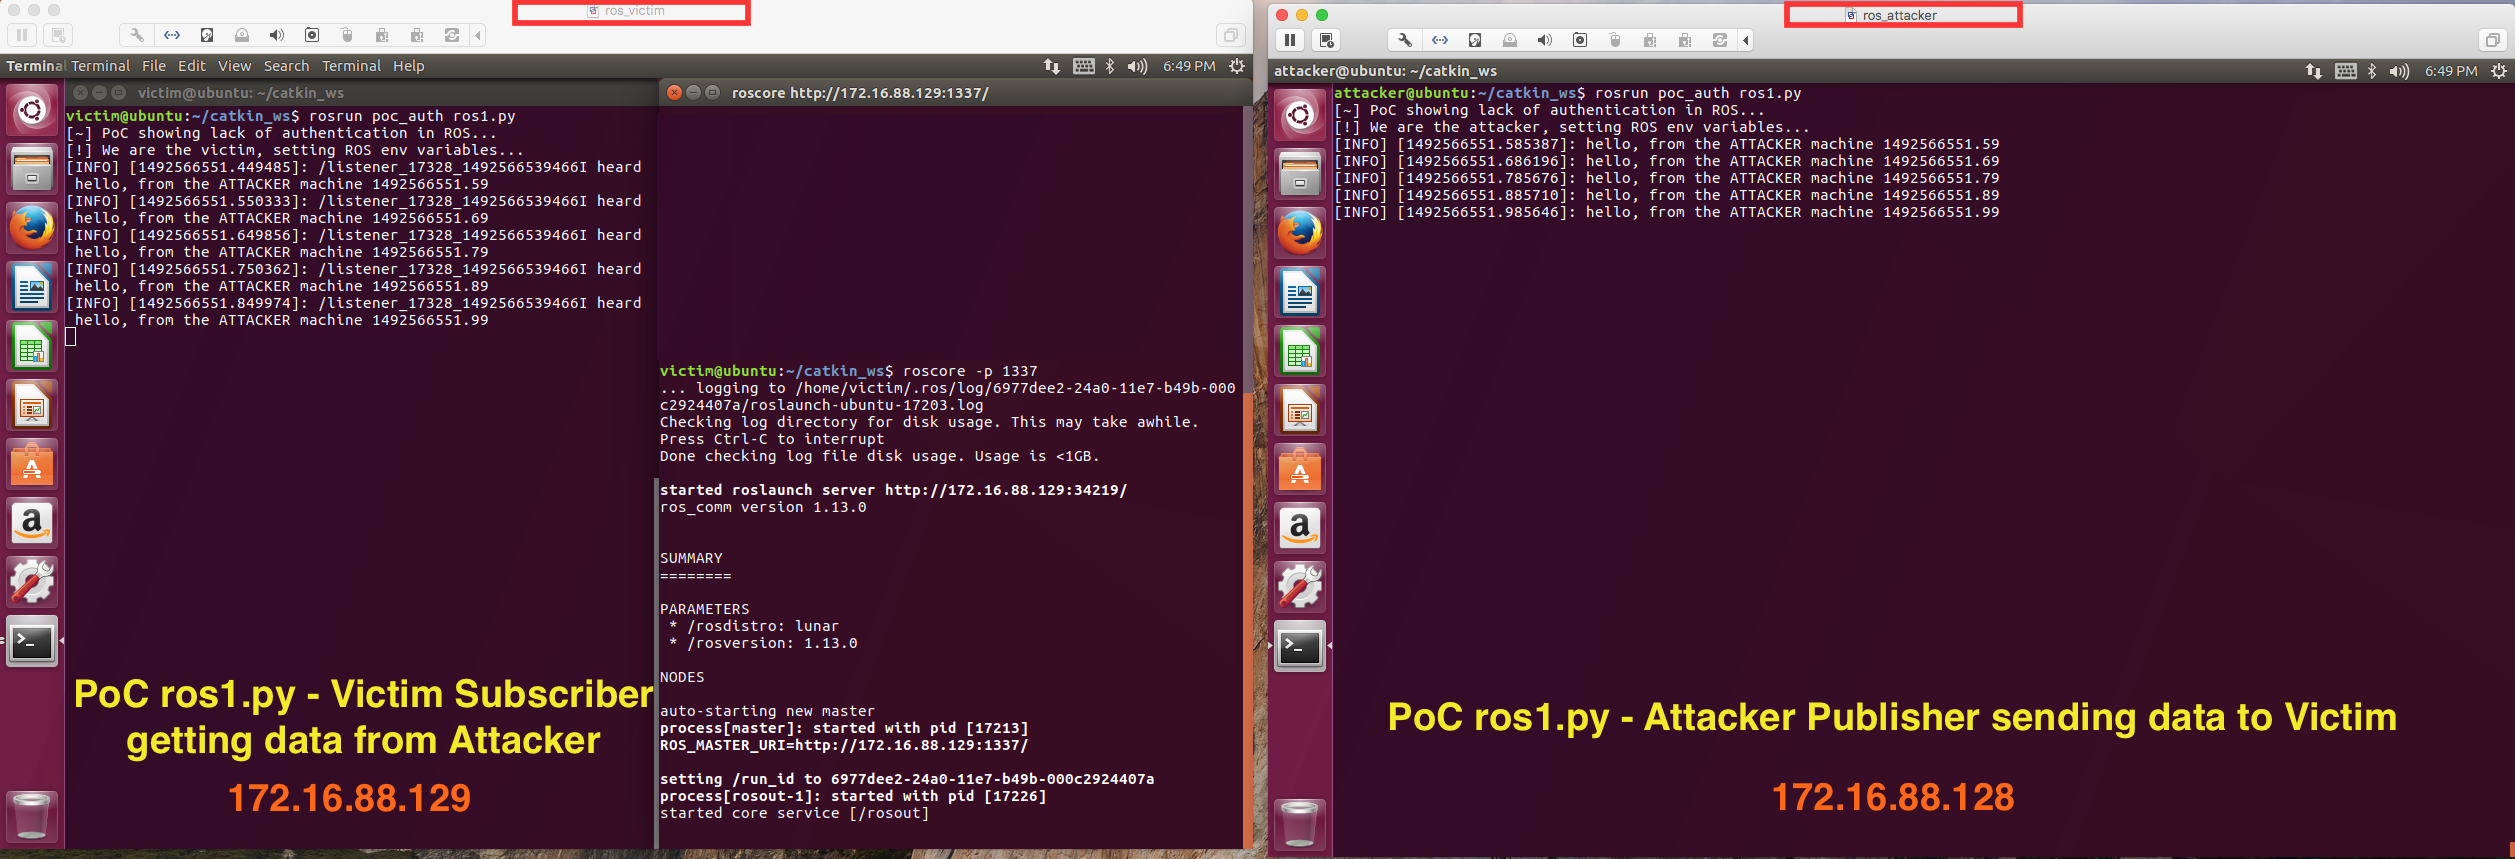
\includegraphics[width=\textwidth]{poc1.eps}
    \caption{PoC ROS Broken Authentication}
\end{figure}

Two PoC packages were created that show ROS has zero authentication measures, by leveraging the publisher subscriber model.
These simple yet effective PoCs are the basis for remote ROS exploitation. If you know the IP address of a remote ROS machine, you can leverage it as you wish, without the need
to authenticate with the machine in any way. This should not be taken lightly, as this opens up ROS to any device that has a network connection. The PoC proving this to be true
connects to a remote "victim" machine, sending data to a ROS subscriber process. This complete PoC package extends upon Malpac 8 and 15. The idea came from expanding upon a study done by a university in South Korea \cite{ROSVulnCounter}.

\subsection{ROS Process Communication}
\begin{figure}[H]
  \centering
    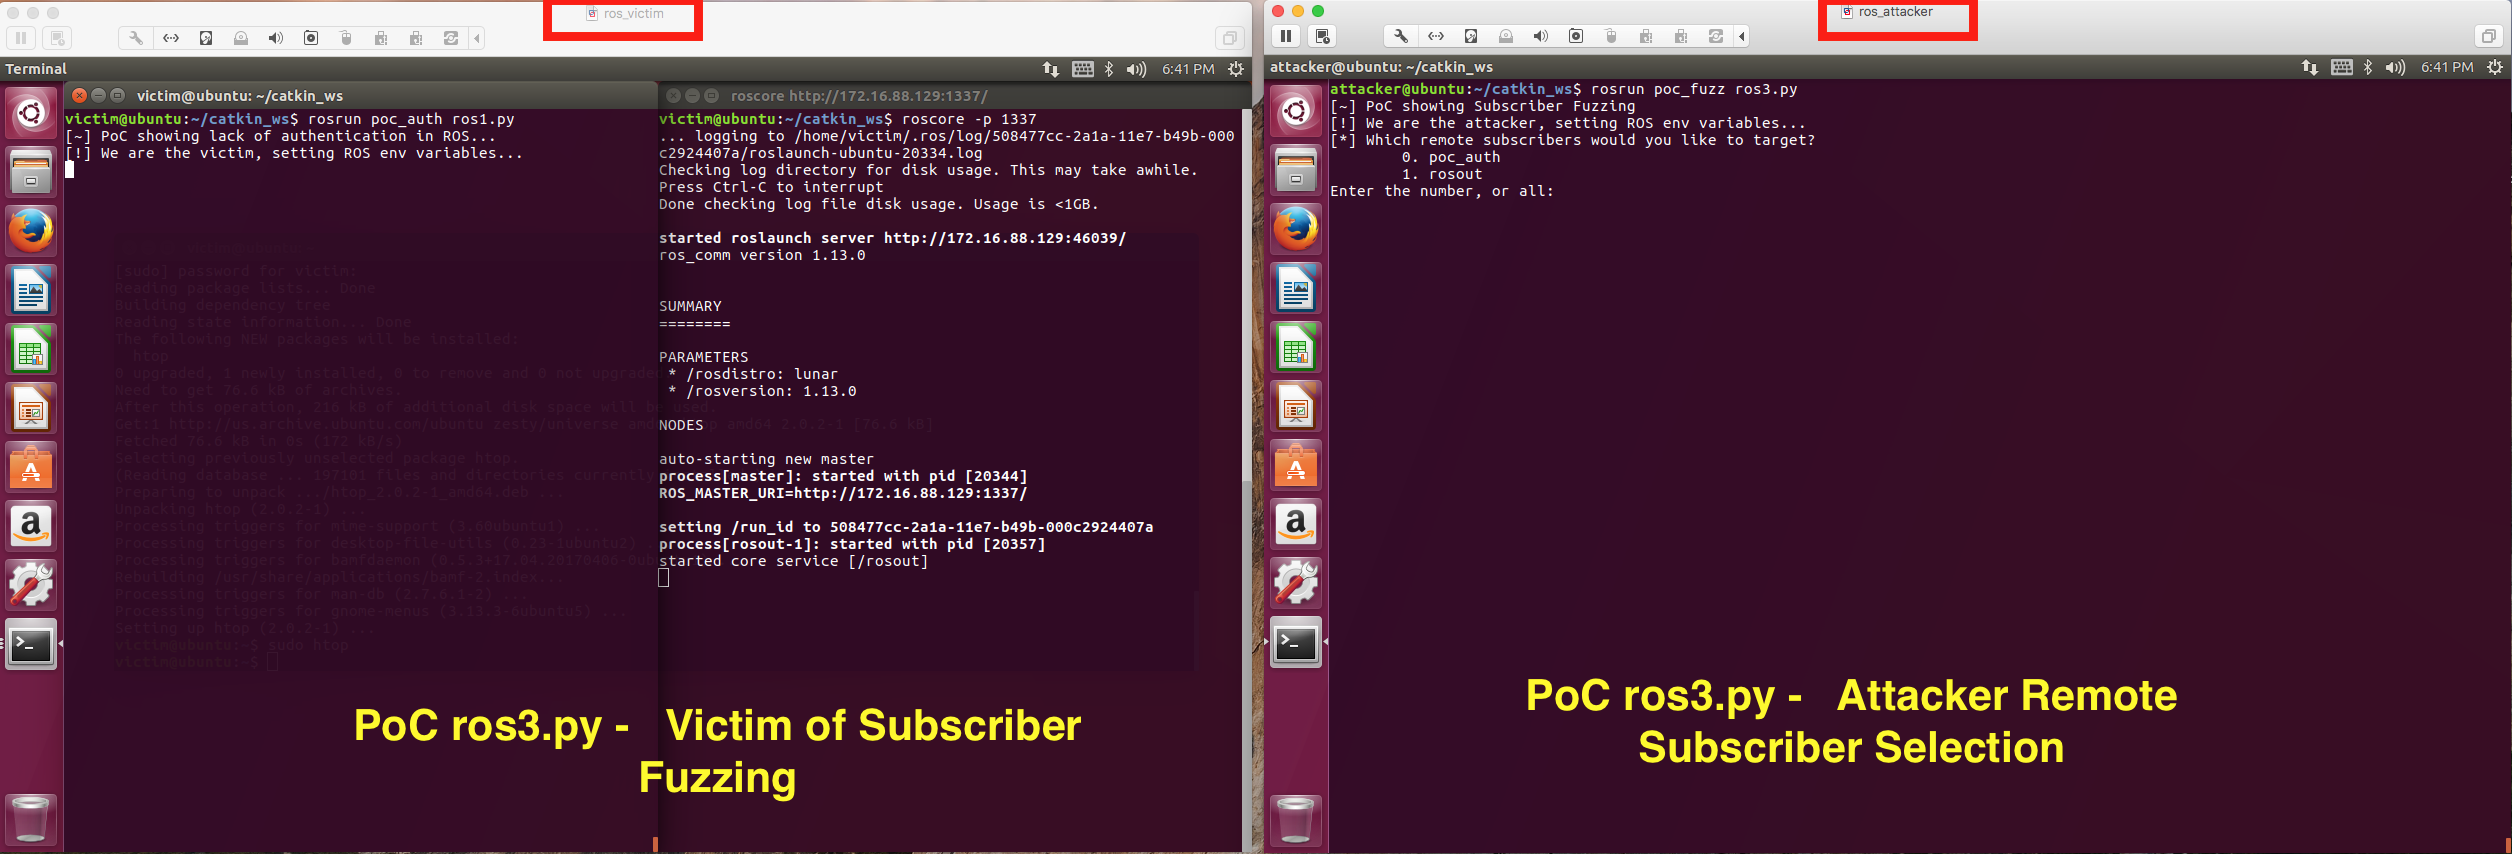
\includegraphics[width=\textwidth]{poc2.eps}
    \caption{PoC ROS Fuzzer Selection}
\end{figure}

Two additional packages were created, exploring exploitation of the process communication model that ROS uses. These PoC packages act as ROS security tools, one of which is a subscriber
fuzzing tool, and the other a publisher data capture tool. The subscriber fuzzer allows an attacker to target remote ROS processes by flooding them with large amounts of malformed data.
This can be used to expose issues with ROS processes on a real world device, like a drone. The idea of creating a fuzzer came from a study that looked at using a similar technique to exploit the MAV Link communicaitons protocol \cite{ROSMAVFuzz}.
The remote publisher data capture tool uses a ROS tool called rosbag to create a saved instance
of a given ROS process. This PoC uses that data to preform what's known as a "ROS Bag Replay Attack", which can cause devices running ROS to carry out a given operation at the will of the attacker.
For example, an attacker could capture what happens with a drone flight control process turns on the motors to begin flight. The attacker could then "replay" that action remotely, causing the drone
to fly. It is also possible to modify this captured data before replaying it via ROS, so an attacker could replay a malicious payload quite easily using this method. The idea of the ROS replay attack came from a
South Korean study \cite{ROSVulnCounter}.

\begin{figure}[H]
  \centering
    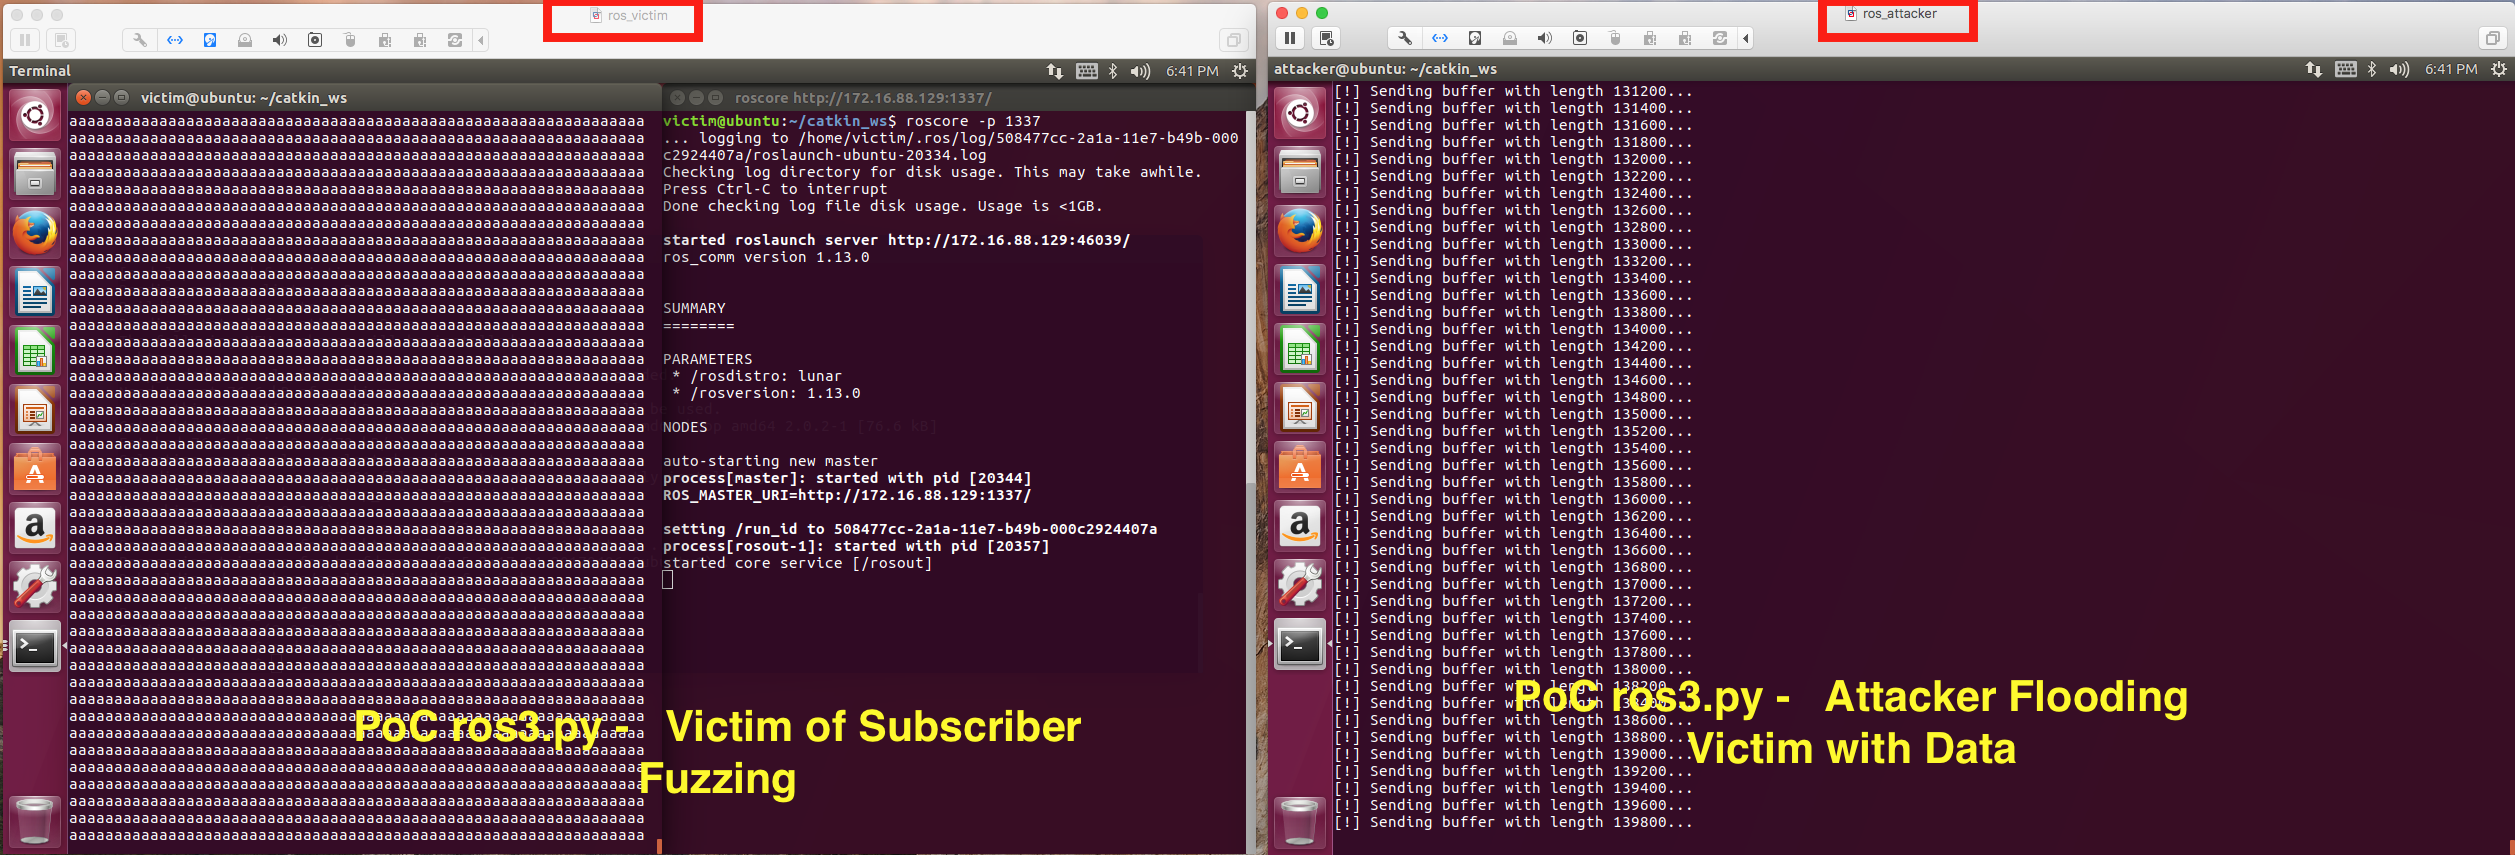
\includegraphics[width=\textwidth]{poc3.eps}
    \caption{PoC ROS Fuzzer Execution}
\end{figure}

\section{Analysis System}
Failure Mode Effects Analysis (FMEA) is a procedure used in a variety of fields which creates an empirical system for testing and logging any failures, which can be applied to all of our attacks. \cite{FMEA}
Somewhat akin to risk analysis, FMEA involves defining severity, occurrence, and detection rating scales, usually from 1 to 10.
After these scales have been defined one can use them to calculate a risk priority number (RPN) and a criticality number with which the found failures can be ranked in order of importance.
You can see this represented in figure 5 below.

\begin{figure}[H]
    \centering
    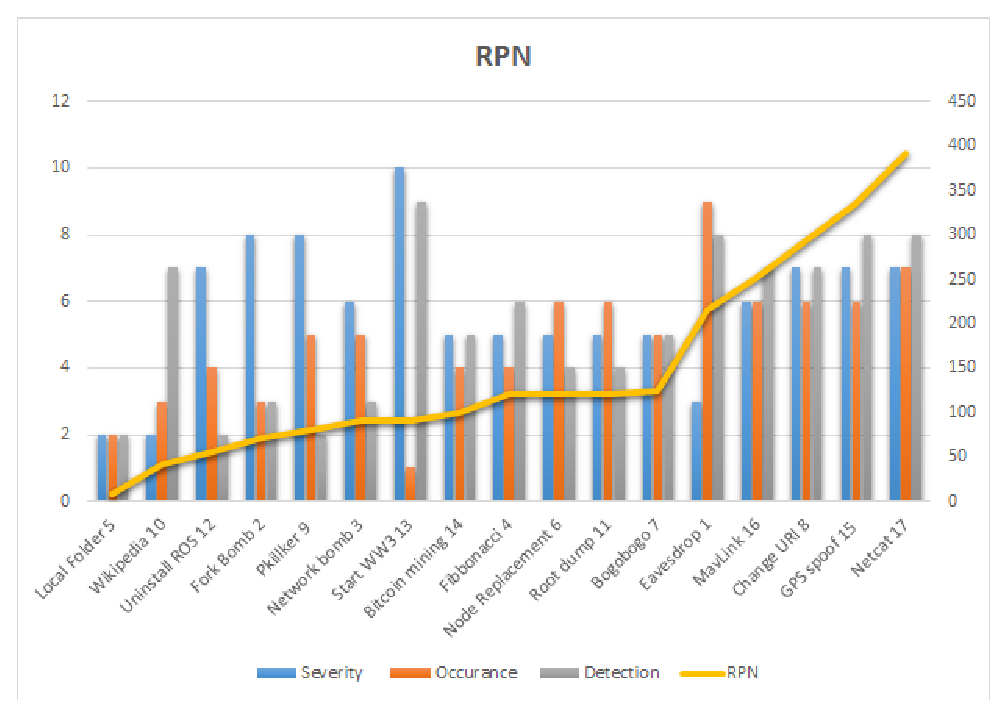
\includegraphics[width=\textwidth]{RPN.eps}
    \caption{The increasing criticality ratings of packages, based on the three combined numbers}
\end{figure}

\section{Findings}
Just as suspected, ROS has wide range of vulnerabilities that this project exploits with a success rate of nearly 100\%.
Most of these exploits involved either entering the system via the publisher/subscriber system that ROS uses to communicate, or demonstrated what malicious actions could take place on the system once inside.
Those that interrupted the availability of the system were most prevalent, since it's somewhat trivial to break subsystems once inside.
The next most common type of exploit was those that tamper with the integrity of data, usually in network communication.
The least common were those that broke the confidentiality of data, often through authentication or sniffing.

We also found that our project evolved as we went along.
We had initially intended to do more hardware based attacks, but they proved to be too cumbersome and difficult to generalize.
There are also a board range of physical attacks ranging anywhere from an EMP type gun to an eagle taking down an airborne drone.

Not every area from the threat model was successful, some were not possible to breach, but it is important to acknowledge their importance.
This new version of the threat model was created to showcase the success level of each area using color coding.
Those areas that are red have a lot more potential for vulnerabilities, yellow has been covered by our research but is still likely to have more, and green was heavily covered and only an expert in that area would be likely to identify more.
This also includes our specific packages as leaves, rather than the general concepts they covered.

\begin{figure}[H]
    \centering
    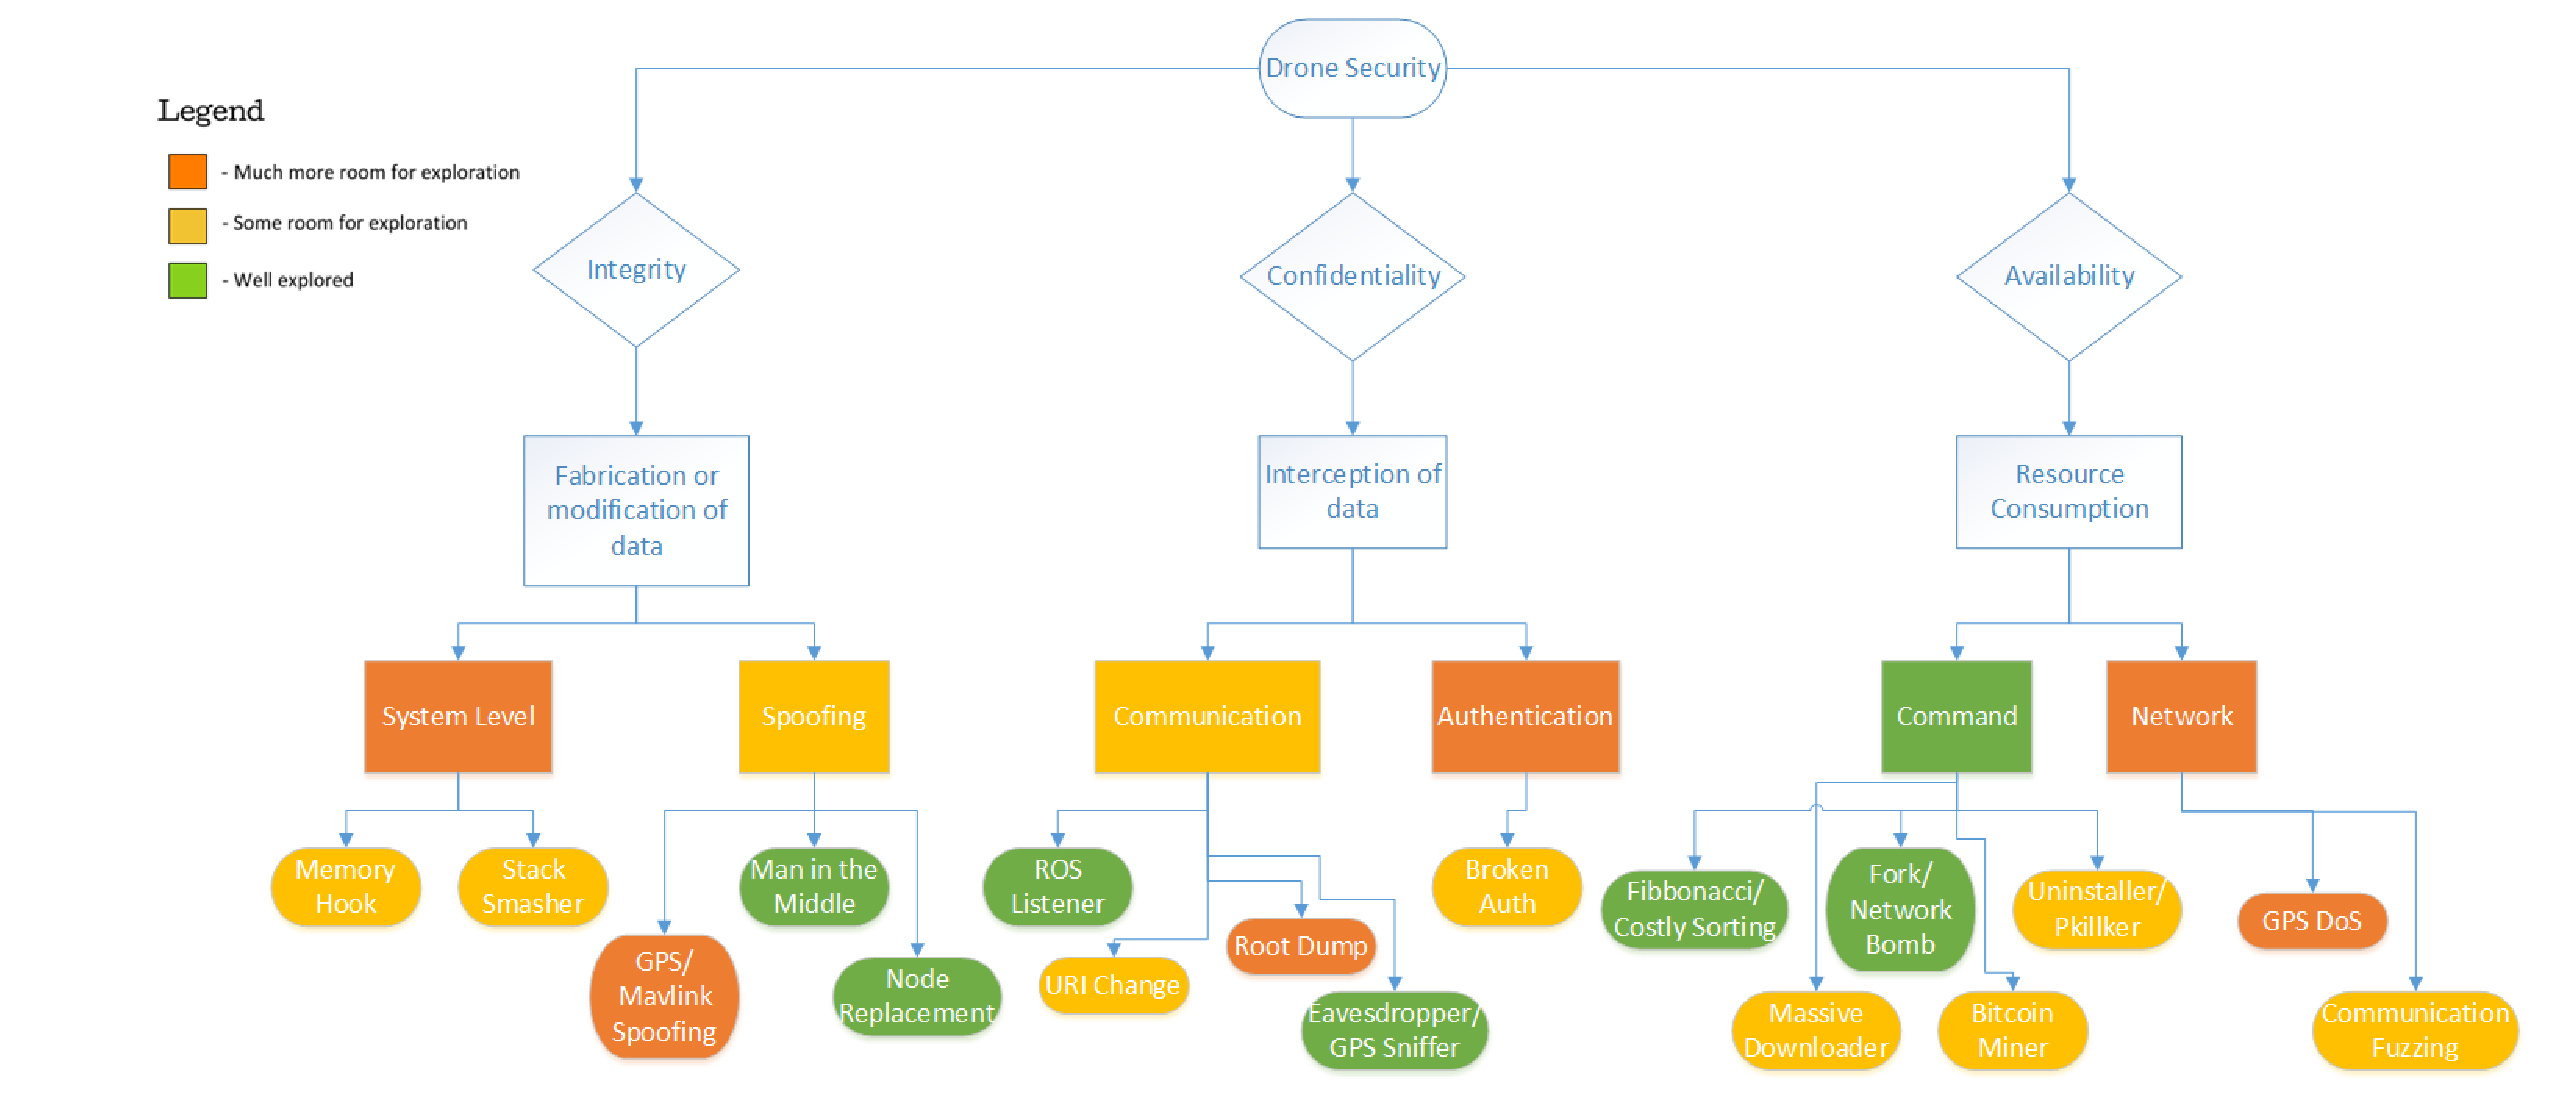
\includegraphics[width=\textwidth]{color_model.eps}
    \caption{map of the areas which were most or least covered in this research}
\end{figure}

\section{Analysis}
As discussed above in the Methods sections, FMEA was used primarily in the analysis of this project, in order to discover which of the created packages would be most catastrophic. 
In the figure above representing the graph of the RPNs, one can see which types of attacks were ranked the highest. 
Those that focused on the integrity of the system turned out to have the highest concentration in the top of that ranking.

There are a number of factors that could have lead to this clustering.
Firstly, the majority of them were more thorough and written in a greater depth than many of those in other categories.
This means that they would be likely ranked more severely since they do more damage in more detail within the scope of this research.
Another potential reason for this is that spoofing and changing of data to something malicious tends to be perceived as more nefarious than something like resource consumption.

Another interesting metric by which to compare the exploits is the time it took to write them.
On average the time to complete an availability package was 18.75 minutes.
For confidentiality the average was 246.7 minutes.
Integrity came in at 296 minutes average development time, which is the longest.
This helps to back up the trend of integrity focused packages being ranked as some of the most severe.
If more time went into the development of them, then it makes sense that they would likely be more sophisticated.

The table from which these averages came can be viewed below.

\begin{center}
\begin{tabular}{ |p{0.3\linewidth}|p{0.3\linewidth}|p{0.3\linewidth}| }
\hline
    Package Name & Primary Type & Time Spent (in Minutes) \\ \hline
    Malpac2 & Availability & 10 \\ \hline
    Malpac3 & Availability & 20 \\ \hline
    Malpac5 & Availability & 5 \\ \hline
    Malpac7 & Availability & 25 \\ \hline
    Malpac9 & Availability & 20 \\ \hline
    Malpac10 & Availability & 20 \\ \hline
    Malpac12 & Availability & 15 \\ \hline
    Malpac14 & Availability & 35 \\ \hline
    Malpac1 & Confidentiality & 30 \\ \hline
    Malpac11 & Confidentiality & 25 \\ \hline
    GPS1 & Confidentiality & 300 \\ \hline
    Malpac\_Coms (nc\_drop.py) & Confidentiality & 720 \\ \hline
    Malpac\_ROS (ros1.py) & Confidentiality & 360 \\ \hline
    Malpac\_ROS (ros2.py) & Confidentiality & 45 \\ \hline
    Malpac6 & Integrity & 40 \\ \hline
    Malpac8 & Integrity & 30 \\ \hline
    Malpac13 & Integrity & 10 \\ \hline
    Malpac15 & Integrity & 300 \\ \hline
    GPS2 & Integrity & 420 \\ \hline
    MavLink & Integrity & 240 \\ \hline
    MemHook & Integrity & 840 \\ \hline
    StackSmash & Integrity & 540 \\ \hline
    Malpac\_ROS (ros3.py) & Integrity & 480 \\ \hline
    Malpac\_ROS (ros4.py) & Integrity & 60 \\ \hline
     &  & \  \\ \hline
\end{tabular}
\end{center} 

\section{Limitations}
The main limitation our project faced was not being able to do testing on actual robotic hardware.
If this project were continued, the next steps would be to setup a ROS enabled drone and see how our exploit packages effect the drone's functionality.
Testing on real world hardware will drive home the real-world implications of using an insecure middleware on robotic devices with open communication channels.
Our research is not just limited to drones; any device running ROS can be used to further test our methods.
While our testing was done on ROS enabled machines, those machines were not real-world robotic devices, thus the real-world impact of our packages could not be evaluated.

If this project had spanned longer than one year there also would have been much more time to expand the breadth and depth of this research.
Keeping our investigations within the scope of both the project requirements and the time constraints was a continuous challenge.

\section{Future Research}

%discuss problems and failures here

There were plans to use real world hardware to test our ROS exploit packages, in this case a drone. However,
we ran into some issues getting our hardware platform to work. This section will try to go through the
hardware that was used, as well as the issues that occurred along the way so that the same mistakes are not
made in the future. Also, where possible, there will be a mention of recommended next steps for anyone
interested in continuing this project.

There were two drones at our disposal, though we really focused our efforts on one of them; the Flame Wheel ARF F550. The other drone we had was a complete, proprietary NazaM2 based drone, with its own micro controller
and flight controller. The Flame Wheel F550 was already hooked up to a Beagle Bone Black, which is the
micro controller we decided to use, so it made sense to focus on the Flame Wheel drone. Along with this
Flame Wheel drone, we had a Beagle Bone Black micro controller, a Pixhawk v1.6 Firecape, and a 3DR compass and
magnetometer radio. The idea was that ROS would be running on the Beagle Bone Black, along with the ArduPilot
project \cite{Ardu}, and the Pixhawk would act as our flight controller. Based on the current
ArduPilot project documentation, the Pixhawk is a supported flight controller \cite{ArduFlightController}.
However, we later found out that our Pixhawk v1.6 was no longer supported, and documentation was incredibly
lacking. Our team recommends that the newer version of the Pixhawk be used instead of the out-dated v1.6.

It should also be mentioned that we were given two Beagle Bone Black micro controllers, and two
Pixhawk v1.6 flight controllers. Only one of the Pixhawks was used, as the other one had damage to the
tty0 connection. We had planned to fix this ourselves, though never got around to it. Also, only one of the
Beagle Bone Blacks was used, as there was no reason to suggest that it had any problems.

\subsection{Why This Hardware Was Used}

We decided to use this hardware as it was available to us and did not require that we purchase anything new.
In terms of why use a drone, we discussed the current trend of drones becoming popular in the hobbyist and
commercial sectors, and thought it be important that our security evaluation of ROS extend to drones that use it. Moving forward, we feel there is no reason to use different drone hardware, as it is our view that the
issues we ran into are related to the micro controller and flight controller. We would highly suggest that
newer versions of the supported micro controllers be used, along with a compatible paired flight controller,
that is still supported by the manufacture and the community. These include, but are not limited to, the
Erle Brain 2, the newer Pixhawks, and more \cite{ArduFlightController}.

Due to the issues we encountered, we were not able to test our exploits on real hardware. Instead, we managed
to lay the ground work needed for future work to be extended to real world hardware, such as drones. It is
our view, that great care and time needs to be taken to find a set of hardware that is currently supported,
and that works with the ROS drone configuration we were hoping to achieve.

\subsection{Beagle Bone Black: Stability, UbuntuARM, and ROS}

The first thing we did with regards to getting our hardware setup was to get a stable operating system
running on the Beagle Bone Black (BBB). We knew that we wanted to run ROS, and according to the ROS
documentation, Ubuntu was the route to go \cite{ROSBBBUbuntu}. To do this, we followed
the extensive documentation to install Ubuntu ARM 16.4, which was the latest Ubuntu ARM build at the time
\cite{eLinuxBBB}.

While flashing Ubuntu on the BBB was pretty easy, we ran into an issue where the BBB would randomly restart
and would enter user flashing mode, even though we flashed Ubuntu to the internal memory. After going through
this process a second time, we managed to get a stable Ubuntu ARM version running on the BBB. The logs for
the internal eMMC flash can be seen on our project GitHub \cite{eMMCLog}. We are not
sure why this did not work the first time, but after a couple weeks made the decision to reflash Ubuntu,
which ended up working as expected.

Once Ubuntu was running, we installed ROS following the online documentation \cite{ROSUbuntuARM}. This process went as expected, and did not present any issues. Once we had ROS running on a stable
Ubuntu build, we moved on to try and get the BBB to detect the Pixhawk v1.6 Firecape.


\subsection{Pixhawk i2c Detection and Beagle Bone Device Trees}

Following along with the ArduPilot documentation, after installing Ubuntu and hooking up the Pixhawk
flight controller, running the 'i2cdetect' command should tell you if the Pixhawk is being detected
by the BBB \cite{PixhawkDetectionArdu}.
When we ran this command, and we did not get the same output \cite{PixhawkDetectLog}, which
told us that the Pixhawk was not yet being read by the Beagle Bone Black. UbuntuARM did not seem to have the
device trees preconfigured for the Pixhawk.

Looking ahead, we found that the ArduPilot project has the device trees needed for the Pixhawk Fire Cape
\cite{ArduGuideDeviceTrees}. We thought that by moving forward with compiling ArduPilot, we would also be working towards getting the Pixhawk operational.


\subsection{Compiling ArduPilot Project}

After installing the needed build tools on UbuntuARM, we proceeded to to pull the latest version of the
ArduPilot project from git, per instructions listed in the documentation \cite{ArduCompileBBB}.

After the code was pulled from the ArduPilot git, we compiled the ArduCopter specific packages, as this is
needed for multi-copter, or hex-copter style drones, which is what our Flame Wheel F550 is. A log from this process can be
seen on our project's GitHub \cite{ArduCompileLog}.

It took a long time to compile the ArduCopter code on the Beagle Bone Black, and all appeared to compile
correctly, without any errors.

We then continued with the instructions on building and enabling the proper Beagle Bone Black device trees
for the Pixhawk Firecape, and enabled the cape manager at the kernel level, per these instructions \cite{ArduGuideDeviceTrees}.

It should be noted, that these build instructions are assuming that the Beagle Bone Black is running a Debian
image, not an Ubuntu image. We continued using the Ubuntu image at this point, as we saw it as needed in order
to get ROS working properly, per the ROS build guide \cite{ROSBBBUbuntu}. It is unclear if
this was the reason for our initial issues with getting the BBB to communicate with the Pixhawk.

\subsection{ArduPilot Pixhawk Detection Issues}

At this point, even after using the device trees from the ArduPilot project, the Pixhawk still was not being
recognized by the Beagle Bone Black. Feeling stuck, we spoke with one of our project mentors, Kevin McGrath,
who suggested we use an "all in one" ArduPilot image, that has everything we need ready to go.
Upon our initial research, we could not find such an image, though luckily our mentor was able to share the
Beagle Bone Black image with us.

It was an old version of the ErleBrain image that supported the Pixhawk Fire v1.6 cape; the current image on
their website is for the Pixhawk Fire Mini and Raspberry Pi. Flashing this image instead of UbuntuARM showed
results immediately. Upon first boot the Pixhawk started to respond to the Beagle Bone Black, and ROS along
with the ArduCopter project was ready to go. We highly suggest that this image be used at as a starting point
in the future, as our group spent well over a month trying to sort through issues with getting the UbuntuARM
image and device trees to work properly. We have a copy of this image on our project GitHub \cite{ErleBrainAIOImage}.

\subsection{Pixhawk Wiring and 3DR GPS Incompatibilities}

According to the ArduCopter documentation, we need to have a Pixhawk flight controller, RC Receiver, 3DR GPS
Unit, an assembled multi-copter drone, and a battery \cite{ArduCopterIntro}.
Since we had all of these, and it appeared we now had a working image flashed on the Beagle Bone Black, we
started the process of hooking everything up, per the directions outlines in
the ArduCopter documentation. This is when we started to run into more problems, as the documentation shows a
wiring guide for a newer version of the Pixhawk flight controller, and not the 1.6 version that we had
\cite{ArduPixhawkWiring}.

One of the primary issues we faced was that there was no port on the Pixhawk that was labeled for the GPS
unit, and our wiring for the 3DR GPS unit did not seem to be compatible with our version of the Pixhawk; after
hooking everything up, there were no open ports on the Pixhawk for the 3DR GPS unit.
After speaking with Kevin McGrath about this issue, he too was puzzled by the 3DR GPS not having a proper
set of wires for our Pixhawk flight controller. He gave us a new wire to use for the 3DR, and we hooked it
up to the only port it could plug into on the Pixhawk, the tty0 port.


\subsection{Pre-flight Saftey Check Failures}

For the sake of testing, we launched the ArduCopter application and it started without any problems, and
signaled that it was ready to communicate with our Mission Planner software. Our mission planner was able to
communicate with the drone, and was able to pull settings from the Pixhawk Fire cape. However it would then
crash due to not being able to complete the pre-flight safety checks. The particular error we got with
regards to this failure was that it was unable to detect our GPS unit. That error message can be seen here,
where others using similar hardware had the same problem. We were not able to fix this, and think it might
be due to the Pixhawk being out of date, though are not positive \cite{3DRError} \cite{3DRError2}. 

It was at this point that our client decided that too much time was being spent trying to get the drone to
work, and that we should focus our efforts on developing ROS packages to explore our threat model. It is our
hope that this information will help to guide any future work on this project, so that the same mistakes are
not made trying to get the Pixhawk configuration to work. We highly recommend that efforts be focused on using
recent flight controllers that are still supported by the ArduPilot project.


\section{Conclusion}
ROS is vulnerable in at least the ways detailed above, and as such is insecure.
There are also vulnerabilities whose existence we are confident of, but were unable to write code to exploit in the given time.
In particular, due to our inability to repair our test drone in time, we were unable to attempt any exploits involving hardware.
Most of the vulnerabilities come from basic design choices and philosophy in ROS itself, and to attempt to fix said vulnerabilities would take fundamental changes and re-designs in ROS.
There are indeed already undertakings to do just that, specifically SROS and ROS2, but overall it is probably better to design drone security around the fact that ROS is insecure, if one chooses to use ROS, than attempt to fix ROS itself.
Many of our vulnerability exploits come from having access to ROS itself or by abusing lax communications security to get into ROS, so just ensuring that the ROS is only accessible by trusted users is enough to prevent most exploits that we have found, although that in itself is a rather big task.

\bibliographystyle{IEEEtran}
\bibliography{research}

\end{document}
